\documentclass[border=0pt]{standalone}
\usepackage{iftex}
\ifPDFTeX
  \usepackage[T1]{fontenc}
  \usepackage{DejaVuSans}
  \renewcommand*\familydefault{\sfdefault}
  \usepackage[italic]{mathastext}
\else
  \usepackage{unicode-math}
  \setmainfont{DejaVuSans.ttf}[BoldFont=DejaVuSans-Bold.ttf,ItalicFont=DejaVuSans-Oblique.ttf,
    BoldItalicFont=DejaVuSans-BoldOblique.ttf]
  \setmathfont{texgyredejavu-math.otf}
\fi
\ifPDFTeX  % one glyph of matplotlib mathtext, by Unicode code point (hex)
  \def\mplchar#1{\ifnum"#1="2212 \ensuremath{-}\else\ifnum"#1="D7 \texttimes\else\char"#1\relax\fi\fi}
\else
  \def\mplchar#1{\char"#1\relax}
\fi
\frenchspacing  % matplotlib puts a normal space after punctuation
\usepackage{pgfplots}
\pgfplotsset{compat=1.18}
% matplotlib marker shapes; \pgfplotmarksize = half the matplotlib marker size
\pgfdeclareplotmark{mpl-o}{\pgfpathcircle{\pgfpointorigin}{\pgfplotmarksize}\pgfusepathqfillstroke}
\pgfdeclareplotmark{mpl-o-open}{\pgfpathcircle{\pgfpointorigin}{\pgfplotmarksize}\pgfusepathqstroke}
\pgfdeclareplotmark{mpl-s}{\pgfpathrectangle{\pgfpoint{-\pgfplotmarksize}{-\pgfplotmarksize}}{\pgfpoint{2\pgfplotmarksize}{2\pgfplotmarksize}}\pgfusepathqfillstroke}
\pgfdeclareplotmark{mpl-s-open}{\pgfpathrectangle{\pgfpoint{-\pgfplotmarksize}{-\pgfplotmarksize}}{\pgfpoint{2\pgfplotmarksize}{2\pgfplotmarksize}}\pgfusepathqstroke}
\def\mpltriangle#1{\pgfpathmoveto{\pgfpoint{0pt}{#1\pgfplotmarksize}}\pgfpathlineto{\pgfpoint{-\pgfplotmarksize}{-#1\pgfplotmarksize}}\pgfpathlineto{\pgfpoint{\pgfplotmarksize}{-#1\pgfplotmarksize}}\pgfpathclose}
\pgfdeclareplotmark{mpl-^}{\mpltriangle{}\pgfusepathqfillstroke}
\pgfdeclareplotmark{mpl-^-open}{\mpltriangle{}\pgfusepathqstroke}
\pgfdeclareplotmark{mpl-v}{\mpltriangle{-}\pgfusepathqfillstroke}
\pgfdeclareplotmark{mpl-v-open}{\mpltriangle{-}\pgfusepathqstroke}
\def\mpldiamond{\pgfpathmoveto{\pgfpoint{0pt}{1.41421\pgfplotmarksize}}\pgfpathlineto{\pgfpoint{-1.41421\pgfplotmarksize}{0pt}}\pgfpathlineto{\pgfpoint{0pt}{-1.41421\pgfplotmarksize}}\pgfpathlineto{\pgfpoint{1.41421\pgfplotmarksize}{0pt}}\pgfpathclose}
\pgfdeclareplotmark{mpl-D}{\mpldiamond\pgfusepathqfillstroke}
\pgfdeclareplotmark{mpl-D-open}{\mpldiamond\pgfusepathqstroke}
\pgfdeclareplotmark{mpl-x}{\pgfpathmoveto{\pgfpoint{-\pgfplotmarksize}{-\pgfplotmarksize}}\pgfpathlineto{\pgfpoint{\pgfplotmarksize}{\pgfplotmarksize}}\pgfpathmoveto{\pgfpoint{-\pgfplotmarksize}{\pgfplotmarksize}}\pgfpathlineto{\pgfpoint{\pgfplotmarksize}{-\pgfplotmarksize}}\pgfsetbuttcap\pgfusepathqstroke}
\pgfdeclareplotmark{mpl-+}{\pgfpathmoveto{\pgfpoint{-\pgfplotmarksize}{0pt}}\pgfpathlineto{\pgfpoint{\pgfplotmarksize}{0pt}}\pgfpathmoveto{\pgfpoint{0pt}{-\pgfplotmarksize}}\pgfpathlineto{\pgfpoint{0pt}{\pgfplotmarksize}}\pgfsetbuttcap\pgfusepathqstroke}
\def\mplplus{\pgfpathmoveto{\pgfpoint{-0.33333\pgfplotmarksize}{-\pgfplotmarksize}}\pgfpathlineto{\pgfpoint{0.33333\pgfplotmarksize}{-\pgfplotmarksize}}\pgfpathlineto{\pgfpoint{0.33333\pgfplotmarksize}{-0.33333\pgfplotmarksize}}\pgfpathlineto{\pgfpoint{\pgfplotmarksize}{-0.33333\pgfplotmarksize}}\pgfpathlineto{\pgfpoint{\pgfplotmarksize}{0.33333\pgfplotmarksize}}\pgfpathlineto{\pgfpoint{0.33333\pgfplotmarksize}{0.33333\pgfplotmarksize}}\pgfpathlineto{\pgfpoint{0.33333\pgfplotmarksize}{\pgfplotmarksize}}\pgfpathlineto{\pgfpoint{-0.33333\pgfplotmarksize}{\pgfplotmarksize}}\pgfpathlineto{\pgfpoint{-0.33333\pgfplotmarksize}{0.33333\pgfplotmarksize}}\pgfpathlineto{\pgfpoint{-\pgfplotmarksize}{0.33333\pgfplotmarksize}}\pgfpathlineto{\pgfpoint{-\pgfplotmarksize}{-0.33333\pgfplotmarksize}}\pgfpathlineto{\pgfpoint{-0.33333\pgfplotmarksize}{-0.33333\pgfplotmarksize}}\pgfpathclose}
\pgfdeclareplotmark{mpl-P}{\mplplus\pgfusepathqfillstroke}
\pgfdeclareplotmark{mpl-P-open}{\mplplus\pgfusepathqstroke}
\def\mplstar{\pgfpathmoveto{\pgfpointpolar{90}{\pgfplotmarksize}}%
  \foreach \i in {1,...,4} {\pgfpathlineto{\pgfpointpolar{90+72*\i-36}{0.381966\pgfplotmarksize}}\pgfpathlineto{\pgfpointpolar{90+72*\i}{\pgfplotmarksize}}}%
  \pgfpathlineto{\pgfpointpolar{54}{0.381966\pgfplotmarksize}}\pgfpathclose}
\pgfdeclareplotmark{mpl-*}{\mplstar\pgfusepathqfillstroke}
\pgfdeclareplotmark{mpl-*-open}{\mplstar\pgfusepathqstroke}
\def\mpltriside#1{\pgfpathmoveto{\pgfpoint{#1\pgfplotmarksize}{0pt}}\pgfpathlineto{\pgfpoint{-#1\pgfplotmarksize}{\pgfplotmarksize}}\pgfpathlineto{\pgfpoint{-#1\pgfplotmarksize}{-\pgfplotmarksize}}\pgfpathclose}
\pgfdeclareplotmark{mpl-<}{\mpltriside{-}\pgfusepathqfillstroke}
\pgfdeclareplotmark{mpl-<-open}{\mpltriside{-}\pgfusepathqstroke}
\pgfdeclareplotmark{mpl->}{\mpltriside{}\pgfusepathqfillstroke}
\pgfdeclareplotmark{mpl->-open}{\mpltriside{}\pgfusepathqstroke}
\def\mplpolygon#1{\pgfpathmoveto{\pgfpointpolar{90}{\pgfplotmarksize}}\foreach \i in {1,...,#1} {\pgfpathlineto{\pgfpointpolar{90+360/#1*\i}{\pgfplotmarksize}}}\pgfpathclose}
\pgfdeclareplotmark{mpl-p}{\mplpolygon{5}\pgfusepathqfillstroke}
\pgfdeclareplotmark{mpl-p-open}{\mplpolygon{5}\pgfusepathqstroke}
\pgfdeclareplotmark{mpl-h}{\mplpolygon{6}\pgfusepathqfillstroke}
\pgfdeclareplotmark{mpl-h-open}{\mplpolygon{6}\pgfusepathqstroke}
\definecolor{mplc0}{HTML}{B0B0B0}
\definecolor{mplc1}{HTML}{000000}
\definecolor{mplc2}{HTML}{1F77B4}
\definecolor{mplc3}{HTML}{D62728}
\definecolor{mplc4}{HTML}{DAA520}
\definecolor{mplc5}{HTML}{9467BD}
\definecolor{mplc6}{HTML}{17BECF}
\definecolor{mplc7}{HTML}{2CA02C}
\begin{document}
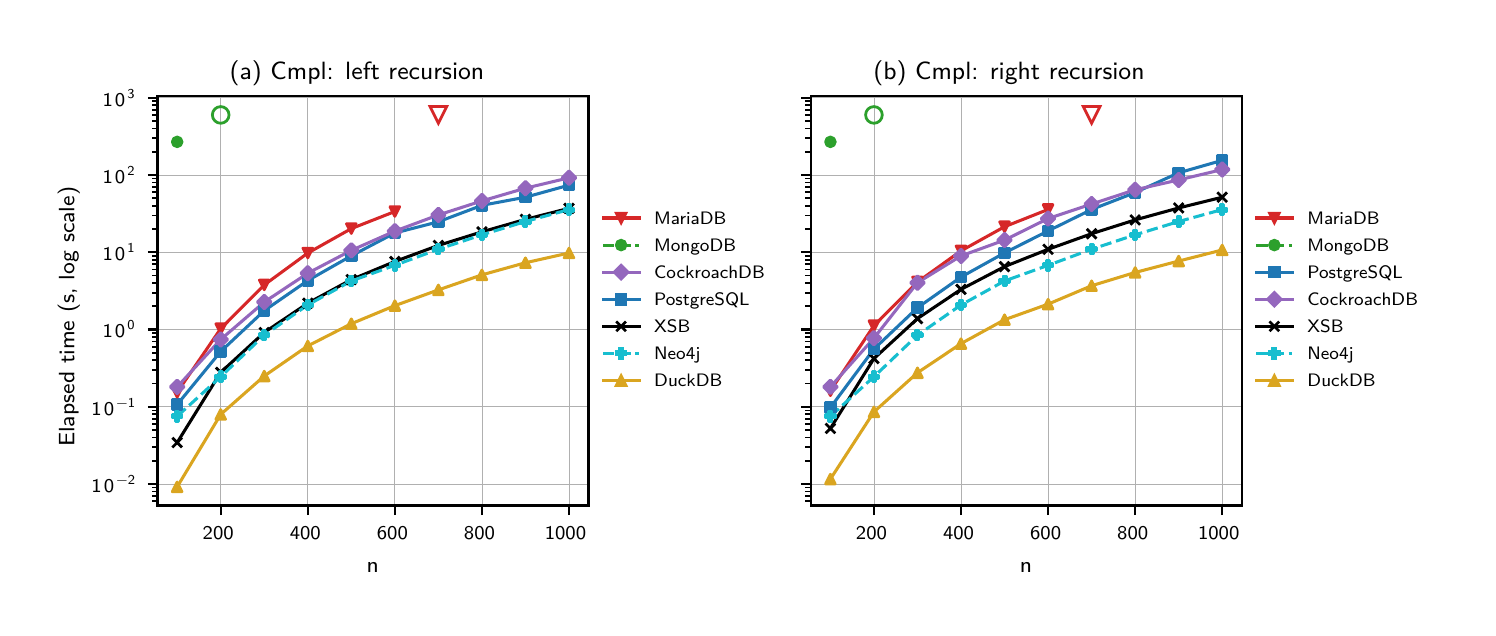
\begin{tikzpicture}
\useasboundingbox (0in,0in) rectangle (7.2in,2.9in);
\begin{axis}[at={(0.6495in,0.5111in)}, anchor=south west, scale only axis, width=2.1552in, height=2.0456in, xmin=55, xmax=1045, ymin=0.005286768138, ymax=1044.392341, enlargelimits=false, clip=true, axis on top=false, axis line style={line width=0.8bp, black}, tick align=outside, tick pos=left, major tick length=3.5bp, minor tick length=2bp, major tick style={line width=0.8bp, black}, minor tick style={line width=0.6bp, black}, xticklabels={}, yticklabels={}, scaled x ticks=false, scaled y ticks=false, xlabel={}, ylabel={}, title={}, xtick={200,400,600,800,1000}, minor xtick={}, ymode=log, log basis y=10, ytick={0.01,0.1,1,10,100,1000}, minor ytick={0.006,0.007,0.008,0.009,0.02,0.03,0.04,0.05,0.06,0.07,0.08,0.09,0.2,0.3,0.4,0.5,0.6,0.7,0.8,0.9,2,3,4,5,6,7,8,9,20,30,40,50,60,70,80,90,200,300,400,500,600,700,800,900}, xmajorgrids, ymajorgrids, major grid style={line width=0.3bp, draw=mplc0}]
\addplot[color=mplc1, line width=1.1bp, line join=round, solid, line cap=rect, mark=mpl-x, mark size=1.75bp, mark options={solid, line width=1bp, draw=mplc1}] coordinates {(100,0.03444538116) (200,0.2790152073) (300,0.9165865898) (400,2.191972971) (500,4.430275583) (600,7.603892231) (700,12.27932801) (800,18.40114298) (900,26.68381219) (1000,37.08715768)};
\addplot[color=mplc2, line width=1.1bp, line join=round, solid, line cap=rect, mark=mpl-s, mark size=1.75bp, mark options={solid, line width=1bp, draw=mplc2, fill=mplc2}] coordinates {(100,0.10700265) (200,0.5202058418) (300,1.755156217) (400,4.309170817) (500,9.000140592) (600,17.78426997) (700,24.84062898) (800,40.54662451) (900,51.66056121) (1000,73.98504692)};
\addplot[color=mplc3, line width=1.1bp, line join=round, solid, line cap=rect, mark=mpl-v, mark size=1.75bp, mark options={solid, line width=1bp, draw=mplc3, fill=mplc3}] coordinates {(100,0.1542943078) (200,1.026941984) (300,3.782338567) (400,9.771712275) (500,20.26457992) (600,33.72164003)};
\addplot[only marks, mark=mpl-v-open, mark size=3bp, mark options={solid, line width=1bp, draw=mplc3}] coordinates {(700,600)};
\addplot[color=mplc4, line width=1.1bp, line join=round, solid, line cap=rect, mark=mpl-^, mark size=1.75bp, mark options={solid, line width=1bp, draw=mplc4, fill=mplc4}] coordinates {(100,0.009202433587) (200,0.07970109981) (300,0.2503041832) (400,0.6138357336) (500,1.189680233) (600,2.03986505) (700,3.260771625) (800,5.105695167) (900,7.32663015) (1000,9.801412734)};
\addplot[color=mplc5, line width=1.1bp, line join=round, solid, line cap=rect, mark=mpl-D, mark size=1.75bp, mark options={solid, line width=1bp, draw=mplc5, fill=mplc5}] coordinates {(100,0.1809808248) (200,0.7439549) (300,2.269960925) (400,5.363995958) (500,10.59631608) (600,18.80425937) (700,30.45049159) (800,46.25074346) (900,67.60210401) (1000,92.07924264)};
\addplot[color=mplc6, line width=1.1bp, line join=round, dash pattern=on 4.07bp off 1.76bp, line cap=butt, mark=mpl-P, mark size=1.75bp, mark options={solid, line width=1bp, draw=mplc6, fill=mplc6}] coordinates {(100,0.07538787501) (200,0.2452723666) (300,0.845489275) (400,2.082864916) (500,4.255795692) (600,6.784530042) (700,10.96191198) (800,16.83425785) (900,25.02958999) (1000,35.74486112)};
\addplot[color=mplc7, line width=1.1bp, line join=round, dash pattern=on 4.07bp off 1.76bp, line cap=butt, mark=mpl-o, mark size=1.75bp, mark options={solid, line width=1bp, draw=mplc7, fill=mplc7}] coordinates {(100,268.8443788)};
\addplot[only marks, mark=mpl-o-open, mark size=3bp, mark options={solid, line width=1bp, draw=mplc7}] coordinates {(200,600)};
\end{axis}
\begin{axis}[at={(3.9157in,0.5111in)}, anchor=south west, scale only axis, width=2.1552in, height=2.0456in, xmin=55, xmax=1045, ymin=0.005286768138, ymax=1044.392341, enlargelimits=false, clip=true, axis on top=false, axis line style={line width=0.8bp, black}, tick align=outside, tick pos=left, major tick length=3.5bp, minor tick length=2bp, major tick style={line width=0.8bp, black}, minor tick style={line width=0.6bp, black}, xticklabels={}, yticklabels={}, scaled x ticks=false, scaled y ticks=false, xlabel={}, ylabel={}, title={}, xtick={200,400,600,800,1000}, minor xtick={}, ymode=log, log basis y=10, ytick={0.01,0.1,1,10,100,1000}, minor ytick={0.006,0.007,0.008,0.009,0.02,0.03,0.04,0.05,0.06,0.07,0.08,0.09,0.2,0.3,0.4,0.5,0.6,0.7,0.8,0.9,2,3,4,5,6,7,8,9,20,30,40,50,60,70,80,90,200,300,400,500,600,700,800,900}, xmajorgrids, ymajorgrids, major grid style={line width=0.3bp, draw=mplc0}]
\addplot[color=mplc1, line width=1.1bp, line join=round, solid, line cap=rect, mark=mpl-x, mark size=1.75bp, mark options={solid, line width=1bp, draw=mplc1}] coordinates {(100,0.05255241394) (200,0.4215001583) (300,1.387761211) (400,3.314581442) (500,6.531657982) (600,10.93264813) (700,17.41327376) (800,26.27130919) (900,37.51010695) (1000,51.64135785)};
\addplot[color=mplc2, line width=1.1bp, line join=round, solid, line cap=rect, mark=mpl-s, mark size=1.75bp, mark options={solid, line width=1bp, draw=mplc2, fill=mplc2}] coordinates {(100,0.0977462162) (200,0.559385925) (300,1.916793975) (400,4.779705458) (500,9.836559083) (600,18.90447296) (700,35.84478488) (800,59.35295901) (900,107.0000605) (1000,154.8314031)};
\addplot[color=mplc3, line width=1.1bp, line join=round, solid, line cap=rect, mark=mpl-v, mark size=1.75bp, mark options={solid, line width=1bp, draw=mplc3, fill=mplc3}] coordinates {(100,0.1615089248) (200,1.123078159) (300,4.128593008) (400,10.44366118) (500,21.44472192) (600,35.84088214)};
\addplot[only marks, mark=mpl-v-open, mark size=3bp, mark options={solid, line width=1bp, draw=mplc3}] coordinates {(700,600)};
\addplot[color=mplc4, line width=1.1bp, line join=round, solid, line cap=rect, mark=mpl-^, mark size=1.75bp, mark options={solid, line width=1bp, draw=mplc4, fill=mplc4}] coordinates {(100,0.01161540019) (200,0.0859994502) (300,0.2759036) (400,0.65790575) (500,1.341179567) (600,2.133468917) (700,3.694464117) (800,5.48536945) (900,7.706397641) (1000,10.71611327)};
\addplot[color=mplc5, line width=1.1bp, line join=round, solid, line cap=rect, mark=mpl-D, mark size=1.75bp, mark options={solid, line width=1bp, draw=mplc5, fill=mplc5}] coordinates {(100,0.1812666666) (200,0.7744398916) (300,4.043811425) (400,8.982510042) (500,14.38758517) (600,27.35941057) (700,42.16238447) (800,64.49728323) (900,86.47415401) (1000,117.7539245)};
\addplot[color=mplc6, line width=1.1bp, line join=round, dash pattern=on 4.07bp off 1.76bp, line cap=butt, mark=mpl-P, mark size=1.75bp, mark options={solid, line width=1bp, draw=mplc6, fill=mplc6}] coordinates {(100,0.07538787501) (200,0.2452723666) (300,0.845489275) (400,2.082864916) (500,4.255795692) (600,6.784530042) (700,10.96191198) (800,16.83425785) (900,25.02958999) (1000,35.74486112)};
\addplot[color=mplc7, line width=1.1bp, line join=round, dash pattern=on 4.07bp off 1.76bp, line cap=butt, mark=mpl-o, mark size=1.75bp, mark options={solid, line width=1bp, draw=mplc7, fill=mplc7}] coordinates {(100,268.8443788)};
\addplot[only marks, mark=mpl-o-open, mark size=3bp, mark options={solid, line width=1bp, draw=mplc7}] coordinates {(200,600)};
\end{axis}
\draw[color=mplc3, line width=1.1bp, line join=round, solid, line cap=rect] (2.8769in,1.9483in) -- (3.0575in,1.9483in);
\begin{scope}[solid, line width=1bp, draw=mplc3, fill=mplc3]\pgftransformshift{\pgfpoint{2.9672in}{1.9483in}}\pgfsetplotmarksize{1.75bp}\pgfuseplotmark{mpl-v}\end{scope}
\draw[color=mplc7, line width=1.1bp, line join=round, dash pattern=on 4.07bp off 1.76bp, line cap=butt] (2.8769in,1.8129in) -- (3.0575in,1.8129in);
\begin{scope}[solid, line width=1bp, draw=mplc7, fill=mplc7]\pgftransformshift{\pgfpoint{2.9672in}{1.8129in}}\pgfsetplotmarksize{1.75bp}\pgfuseplotmark{mpl-o}\end{scope}
\draw[color=mplc5, line width=1.1bp, line join=round, solid, line cap=rect] (2.8769in,1.6775in) -- (3.0575in,1.6775in);
\begin{scope}[solid, line width=1bp, draw=mplc5, fill=mplc5]\pgftransformshift{\pgfpoint{2.9672in}{1.6775in}}\pgfsetplotmarksize{1.75bp}\pgfuseplotmark{mpl-D}\end{scope}
\draw[color=mplc2, line width=1.1bp, line join=round, solid, line cap=rect] (2.8769in,1.542in) -- (3.0575in,1.542in);
\begin{scope}[solid, line width=1bp, draw=mplc2, fill=mplc2]\pgftransformshift{\pgfpoint{2.9672in}{1.542in}}\pgfsetplotmarksize{1.75bp}\pgfuseplotmark{mpl-s}\end{scope}
\draw[color=mplc1, line width=1.1bp, line join=round, solid, line cap=rect] (2.8769in,1.4066in) -- (3.0575in,1.4066in);
\begin{scope}[solid, line width=1bp, draw=mplc1]\pgftransformshift{\pgfpoint{2.9672in}{1.4066in}}\pgfsetplotmarksize{1.75bp}\pgfuseplotmark{mpl-x}\end{scope}
\draw[color=mplc6, line width=1.1bp, line join=round, dash pattern=on 4.07bp off 1.76bp, line cap=butt] (2.8769in,1.2712in) -- (3.0575in,1.2712in);
\begin{scope}[solid, line width=1bp, draw=mplc6, fill=mplc6]\pgftransformshift{\pgfpoint{2.9672in}{1.2712in}}\pgfsetplotmarksize{1.75bp}\pgfuseplotmark{mpl-P}\end{scope}
\draw[color=mplc4, line width=1.1bp, line join=round, solid, line cap=rect] (2.8769in,1.1358in) -- (3.0575in,1.1358in);
\begin{scope}[solid, line width=1bp, draw=mplc4, fill=mplc4]\pgftransformshift{\pgfpoint{2.9672in}{1.1358in}}\pgfsetplotmarksize{1.75bp}\pgfuseplotmark{mpl-^}\end{scope}
\draw[color=mplc3, line width=1.1bp, line join=round, solid, line cap=rect] (6.1431in,1.9483in) -- (6.3237in,1.9483in);
\begin{scope}[solid, line width=1bp, draw=mplc3, fill=mplc3]\pgftransformshift{\pgfpoint{6.2334in}{1.9483in}}\pgfsetplotmarksize{1.75bp}\pgfuseplotmark{mpl-v}\end{scope}
\draw[color=mplc7, line width=1.1bp, line join=round, dash pattern=on 4.07bp off 1.76bp, line cap=butt] (6.1431in,1.8129in) -- (6.3237in,1.8129in);
\begin{scope}[solid, line width=1bp, draw=mplc7, fill=mplc7]\pgftransformshift{\pgfpoint{6.2334in}{1.8129in}}\pgfsetplotmarksize{1.75bp}\pgfuseplotmark{mpl-o}\end{scope}
\draw[color=mplc2, line width=1.1bp, line join=round, solid, line cap=rect] (6.1431in,1.6775in) -- (6.3237in,1.6775in);
\begin{scope}[solid, line width=1bp, draw=mplc2, fill=mplc2]\pgftransformshift{\pgfpoint{6.2334in}{1.6775in}}\pgfsetplotmarksize{1.75bp}\pgfuseplotmark{mpl-s}\end{scope}
\draw[color=mplc5, line width=1.1bp, line join=round, solid, line cap=rect] (6.1431in,1.542in) -- (6.3237in,1.542in);
\begin{scope}[solid, line width=1bp, draw=mplc5, fill=mplc5]\pgftransformshift{\pgfpoint{6.2334in}{1.542in}}\pgfsetplotmarksize{1.75bp}\pgfuseplotmark{mpl-D}\end{scope}
\draw[color=mplc1, line width=1.1bp, line join=round, solid, line cap=rect] (6.1431in,1.4066in) -- (6.3237in,1.4066in);
\begin{scope}[solid, line width=1bp, draw=mplc1]\pgftransformshift{\pgfpoint{6.2334in}{1.4066in}}\pgfsetplotmarksize{1.75bp}\pgfuseplotmark{mpl-x}\end{scope}
\draw[color=mplc6, line width=1.1bp, line join=round, dash pattern=on 4.07bp off 1.76bp, line cap=butt] (6.1431in,1.2712in) -- (6.3237in,1.2712in);
\begin{scope}[solid, line width=1bp, draw=mplc6, fill=mplc6]\pgftransformshift{\pgfpoint{6.2334in}{1.2712in}}\pgfsetplotmarksize{1.75bp}\pgfuseplotmark{mpl-P}\end{scope}
\draw[color=mplc4, line width=1.1bp, line join=round, solid, line cap=rect] (6.1431in,1.1358in) -- (6.3237in,1.1358in);
\begin{scope}[solid, line width=1bp, draw=mplc4, fill=mplc4]\pgftransformshift{\pgfpoint{6.2334in}{1.1358in}}\pgfsetplotmarksize{1.75bp}\pgfuseplotmark{mpl-^}\end{scope}
\node[anchor=base west, inner sep=0pt, text=mplc1, font=\fontsize{7bp}{8.4bp}\selectfont] at (0.8724in,0.34in) {200};
\node[anchor=base west, inner sep=0pt, text=mplc1, font=\fontsize{7bp}{8.4bp}\selectfont] at (1.3078in,0.34in) {400};
\node[anchor=base west, inner sep=0pt, text=mplc1, font=\fontsize{7bp}{8.4bp}\selectfont] at (1.7432in,0.34in) {600};
\node[anchor=base west, inner sep=0pt, text=mplc1, font=\fontsize{7bp}{8.4bp}\selectfont] at (2.1785in,0.34in) {800};
\node[anchor=base west, inner sep=0pt, text=mplc1, font=\fontsize{7bp}{8.4bp}\selectfont] at (2.583in,0.34in) {1000};
\node[anchor=base west, inner sep=0pt, text=mplc1, font=\fontsize{8bp}{9.6bp}\selectfont] at (1.6918in,0.1767in) {n};
\node[anchor=base west, inner sep=0pt, text=mplc1, font=\fontsize{7bp}{8.4bp}\selectfont] at (0.3161in,0.5759in) {\mplchar{31}};
\node[anchor=base west, inner sep=0pt, text=mplc1, font=\fontsize{7bp}{8.4bp}\selectfont] at (0.378in,0.5759in) {\mplchar{30}};
\node[anchor=base west, inner sep=0pt, text=mplc1, font=\fontsize{4.9bp}{5.88bp}\selectfont] at (0.4408in,0.6161in) {\mplchar{2212}};
\node[anchor=base west, inner sep=0pt, text=mplc1, font=\fontsize{4.9bp}{5.88bp}\selectfont] at (0.4978in,0.6161in) {\mplchar{32}};
\node[anchor=base west, inner sep=0pt, text=mplc1, font=\fontsize{7bp}{8.4bp}\selectfont] at (0.3161in,0.9631in) {\mplchar{31}};
\node[anchor=base west, inner sep=0pt, text=mplc1, font=\fontsize{7bp}{8.4bp}\selectfont] at (0.378in,0.9631in) {\mplchar{30}};
\node[anchor=base west, inner sep=0pt, text=mplc1, font=\fontsize{4.9bp}{5.88bp}\selectfont] at (0.4408in,1.0032in) {\mplchar{2212}};
\node[anchor=base west, inner sep=0pt, text=mplc1, font=\fontsize{4.9bp}{5.88bp}\selectfont] at (0.4978in,1.0032in) {\mplchar{31}};
\node[anchor=base west, inner sep=0pt, text=mplc1, font=\fontsize{7bp}{8.4bp}\selectfont] at (0.3717in,1.3484in) {\mplchar{31}};
\node[anchor=base west, inner sep=0pt, text=mplc1, font=\fontsize{7bp}{8.4bp}\selectfont] at (0.4335in,1.3484in) {\mplchar{30}};
\node[anchor=base west, inner sep=0pt, text=mplc1, font=\fontsize{4.9bp}{5.88bp}\selectfont] at (0.4963in,1.3886in) {\mplchar{30}};
\node[anchor=base west, inner sep=0pt, text=mplc1, font=\fontsize{7bp}{8.4bp}\selectfont] at (0.3717in,1.7356in) {\mplchar{31}};
\node[anchor=base west, inner sep=0pt, text=mplc1, font=\fontsize{7bp}{8.4bp}\selectfont] at (0.4335in,1.7356in) {\mplchar{30}};
\node[anchor=base west, inner sep=0pt, text=mplc1, font=\fontsize{4.9bp}{5.88bp}\selectfont] at (0.4963in,1.7758in) {\mplchar{31}};
\node[anchor=base west, inner sep=0pt, text=mplc1, font=\fontsize{7bp}{8.4bp}\selectfont] at (0.3717in,2.121in) {\mplchar{31}};
\node[anchor=base west, inner sep=0pt, text=mplc1, font=\fontsize{7bp}{8.4bp}\selectfont] at (0.4335in,2.121in) {\mplchar{30}};
\node[anchor=base west, inner sep=0pt, text=mplc1, font=\fontsize{4.9bp}{5.88bp}\selectfont] at (0.4963in,2.1611in) {\mplchar{32}};
\node[anchor=base west, inner sep=0pt, text=mplc1, font=\fontsize{7bp}{8.4bp}\selectfont] at (0.3717in,2.5073in) {\mplchar{31}};
\node[anchor=base west, inner sep=0pt, text=mplc1, font=\fontsize{7bp}{8.4bp}\selectfont] at (0.4335in,2.5073in) {\mplchar{30}};
\node[anchor=base west, inner sep=0pt, text=mplc1, font=\fontsize{4.9bp}{5.88bp}\selectfont] at (0.4963in,2.5474in) {\mplchar{33}};
\node[anchor=base west, inner sep=0pt, rotate=90, text=mplc1, font=\fontsize{8bp}{9.6bp}\selectfont] at (0.2339in,0.8014in) {Elapsed time (s, log scale)};
\node[anchor=base west, inner sep=0pt, text=mplc1, font=\fontsize{9bp}{10.8bp}\selectfont] at (1.0064in,2.64in) {(a) Cmpl: left recursion};
\node[anchor=base west, inner sep=0pt, text=mplc1, font=\fontsize{6.5bp}{7.8bp}\selectfont] at (3.1297in,1.9167in) {MariaDB};
\node[anchor=base west, inner sep=0pt, text=mplc1, font=\fontsize{6.5bp}{7.8bp}\selectfont] at (3.1297in,1.7813in) {MongoDB};
\node[anchor=base west, inner sep=0pt, text=mplc1, font=\fontsize{6.5bp}{7.8bp}\selectfont] at (3.1297in,1.6459in) {CockroachDB};
\node[anchor=base west, inner sep=0pt, text=mplc1, font=\fontsize{6.5bp}{7.8bp}\selectfont] at (3.1297in,1.5104in) {PostgreSQL};
\node[anchor=base west, inner sep=0pt, text=mplc1, font=\fontsize{6.5bp}{7.8bp}\selectfont] at (3.1297in,1.375in) {XSB};
\node[anchor=base west, inner sep=0pt, text=mplc1, font=\fontsize{6.5bp}{7.8bp}\selectfont] at (3.1297in,1.2396in) {Neo4j};
\node[anchor=base west, inner sep=0pt, text=mplc1, font=\fontsize{6.5bp}{7.8bp}\selectfont] at (3.1297in,1.1042in) {DuckDB};
\node[anchor=base west, inner sep=0pt, text=mplc1, font=\fontsize{7bp}{8.4bp}\selectfont] at (4.1386in,0.34in) {200};
\node[anchor=base west, inner sep=0pt, text=mplc1, font=\fontsize{7bp}{8.4bp}\selectfont] at (4.574in,0.34in) {400};
\node[anchor=base west, inner sep=0pt, text=mplc1, font=\fontsize{7bp}{8.4bp}\selectfont] at (5.0094in,0.34in) {600};
\node[anchor=base west, inner sep=0pt, text=mplc1, font=\fontsize{7bp}{8.4bp}\selectfont] at (5.4448in,0.34in) {800};
\node[anchor=base west, inner sep=0pt, text=mplc1, font=\fontsize{7bp}{8.4bp}\selectfont] at (5.8493in,0.34in) {1000};
\node[anchor=base west, inner sep=0pt, text=mplc1, font=\fontsize{8bp}{9.6bp}\selectfont] at (4.958in,0.1767in) {n};
\node[anchor=base west, inner sep=0pt, text=mplc1, font=\fontsize{9bp}{10.8bp}\selectfont] at (4.2255in,2.64in) {(b) Cmpl: right recursion};
\node[anchor=base west, inner sep=0pt, text=mplc1, font=\fontsize{6.5bp}{7.8bp}\selectfont] at (6.3959in,1.9167in) {MariaDB};
\node[anchor=base west, inner sep=0pt, text=mplc1, font=\fontsize{6.5bp}{7.8bp}\selectfont] at (6.3959in,1.7813in) {MongoDB};
\node[anchor=base west, inner sep=0pt, text=mplc1, font=\fontsize{6.5bp}{7.8bp}\selectfont] at (6.3959in,1.6459in) {PostgreSQL};
\node[anchor=base west, inner sep=0pt, text=mplc1, font=\fontsize{6.5bp}{7.8bp}\selectfont] at (6.3959in,1.5104in) {CockroachDB};
\node[anchor=base west, inner sep=0pt, text=mplc1, font=\fontsize{6.5bp}{7.8bp}\selectfont] at (6.3959in,1.375in) {XSB};
\node[anchor=base west, inner sep=0pt, text=mplc1, font=\fontsize{6.5bp}{7.8bp}\selectfont] at (6.3959in,1.2396in) {Neo4j};
\node[anchor=base west, inner sep=0pt, text=mplc1, font=\fontsize{6.5bp}{7.8bp}\selectfont] at (6.3959in,1.1042in) {DuckDB};
\end{tikzpicture}
\end{document}
